\documentclass[a4paper,11pt]{extarticle}

\usepackage[default]{comfortaa}
\usepackage[utf8]{inputenc}
\usepackage[T1]{fontenc}
\usepackage[english]{babel}
\usepackage[left=0cm, right=0.5cm, bottom=0.5cm, top=0.5cm]{geometry}
\usepackage{fixltx2e}
\usepackage{graphicx}
\usepackage{amsmath}
\usepackage{amssymb}
\usepackage{mathrsfs}
\usepackage{indentfirst}
\usepackage[shortlabels]{enumitem}
\usepackage[usenames,dvipsnames]{xcolor}
\usepackage{tcolorbox}
\usepackage{marvosym}
\usepackage{hyperref}
\usepackage{fontawesome5}

% Background Color of the Sidebar Column and titles
\definecolor{sidebg}{cmyk}{1, 0.02, 0, 0.56}
% Border color of the siderbar and titles
\definecolor{sidefg}{cmyk}{1, 0.02, 0, 0.8}
% Background Color of the Main Column
\definecolor{mainbg}{cmyk}{0, 0, 0.07, 0.04}
% Text Color of the Main Column
\definecolor{maintext}{cmyk}{1, 0.02, 0, 0.8}
% Text Color of the Sidebar Column
\definecolor{sidetext}{cmyk}{0, 0, 0.07, 0.04}

% \colorlet{bgcol}{LimeGreen}
% \colorlet{fgcol}{ForestGreen}
\newcommand{\circb}[1]{\begin{minipage}{1cm}
    \begin{tcolorbox}[colback=sidefg,colframe=sidefg,coltext=sidetext,
        halign=flush center, valign=center, square, circular arc,
        width=0.8cm, left=0cm, right=0cm]
        {\large #1}
    \end{tcolorbox}
\end{minipage}}
\newcommand{\cvtitle}[1]{
    \begin{tcolorbox}[colback=sidebg,colframe=sidefg,coltext=sidetext,
        height=1cm, valign=center, sharp corners=downhill]
        {\Large #1}
    \end{tcolorbox}
}
\newcommand{\gritem}{\color{sidebg}$\blacksquare$}
\renewcommand{\labelitemi}{\gritem}
\newcommand{\griitem}{\color{sidebg}$\blacktriangleright$}
\renewcommand{\labelitemii}{\griitem}
\newcommand{\myspace}{{\color{LimeGreen}\dotfill}}

\renewcommand{\wp}[1]  {\begin{minipage}[b][2mm][c]{3mm} #1 \end{minipage}}
\colorlet{skcol}{OliveGreen}
\colorlet{noskcol}{LimeGreen}
\newcommand{\skdabb} {\colorbox{ForestGreen!80!white}{\color{skcol}$\blacksquare$~\color{noskcol}$\blacksquare$~\color{noskcol}$\blacksquare$}}
\newcommand{\skmore} {\colorbox{ForestGreen!80!white}{\color{skcol}$\blacksquare$~\color{skcol}$\blacksquare$~\color{noskcol}$\blacksquare$}}
\newcommand{\skexp}  {\colorbox{ForestGreen!80!white}{\color{skcol}$\blacksquare$~\color{skcol}$\blacksquare$~\color{skcol}$\blacksquare$}}

\newcommand{\lang}[2]{\hfill \textsc{\scriptsize #1, \textasciitilde#2Sloc}}
\newcommand{\director}[1]{\hfill {\scriptsize #1}}

\begin{document}

\begin{minipage}[c]{0.35\linewidth}
    \begin{tcolorbox}[
        colback=sidebg,
        colframe=sidefg,
        coltext=sidetext,
        subtitle style={
            colback=sidebg,
            coltext=sidetext
        },
        leftrule=2mm,
        sharp corners=uphill,
        height=282mm,
    ]
        \begin{minipage}{0.45\linewidth}
            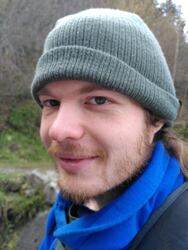
\includegraphics[width=\linewidth]{head.jpg}
        \end{minipage}
        \hfill
        \begin{minipage}{0.45\linewidth}
            Luc

            \textbf{Chabassier}
        \end{minipage}

        \vspace{0.2cm}
        {\small
        \circb{\textborn} September 19, 1996 \newline
        \circb{\Telefon} +33~(0)609642210 \newline
        \circb{\Letter} \href{mailto:luc@dwarfmaster.net}{luc@dwarfmaster.net} \newline
        \circb{\Mundus} \href{https://dwarfmaster.net}{dwarfmaster.net} \newline
        \circb{\faGithub} \href{https://github.com/dwarfmaster}{dwarfmaster} \newline
        }

        \vspace{0.3cm}
        \tcbsubtitle{\Large\bf Interests}

        Programming, Type Theory, Proof Assistants,
        Abstract Interpretation, Formal Systems


        \vspace{0.3cm}
        \tcbsubtitle{\Large\bf Skills}
        \begin{description}\setlength{\itemsep}{0em}
          \item[C++]\hfill\skexp
          \item[Rust]\hfill\skexp
          \item[Shell]\hfill\skexp
          \item[Nix]\hfill\skexp
          \item[Haskell]\hfill\skmore
          \item[\LaTeX]\hfill\skmore
          \item[Coq]\hfill\skmore
          \item[Prolog]\hfill\skmore
          \item[OCaml]\hfill\skmore
          \item[Python]\hfill\skdabb
        \end{description}

        \vspace{0cm}
        \tcbsubtitle{\Large\bf Languages}

        Native french, fluent english, basic spanish


    \end{tcolorbox}\end{minipage}
    \hfill
    \begin{minipage}[c][282mm][t]{0.60\linewidth}
      \pagecolor{mainbg}
      \color{maintext}{

        \cvtitle{Education}

        \begin{itemize}
          \itemsep0em
          \item \emph{Pierre de Fermat} in Toulouse:
                \begin{itemize}[topsep=0em]
                  \itemsep0em
                  \item \textbf{2014} baccalauréat S with highest honours
                  \item \textbf{2014-2016} Maths-Physic preparatory class
                \end{itemize}
          \item \emph{École Normale Supérieure} in Paris:
                \begin{itemize}[topsep=0em]
                  \itemsep0em
                  \item \textbf{2016-2017} Computer science bacherlor's degree
                  \item \textbf{2017-2018} First year of computer science master's degree
                  \item \textbf{2018-2019} Mathematics bahelor's degree
                  \item \textbf{2020-2021} MPRI: Second year of computer science master's degree
                \end{itemize}
        \end{itemize}

        \cvtitle{Professional Experiences}

        \begin{itemize}
          \itemsep0em
          \item \emph{\small (2017)} \textbf{2 months research internship}
                \lang{$\lambda$Prolog}{1k}\\
                A deriving mecanism for Coq
                \director{Enrico Tassi} \\
                MARELLE team at INRIA Sophia-Antipolis
          \item \emph{\small (2018)} \textbf{5 months research internship}
                \lang{CL/Haskell/C++}{3k}\\
                Infering frames semantics
                \director{Marie-Claude L'Homme}\\
                Département de linguistique à UdeM
          \item \emph{\small (2019)} \textbf{\href{https://github.com/dwarfmaster/memoire-dma-l3}{Maths dissertation}}
                \lang{\LaTeX}{4k}\\
                Category theoretic approach to CSPs
                \director{Damianno Mazza}
          \item \emph{\small (2019-2020)} \textbf{5.5 months internship}
                \lang{C++}{5k}\\
                Static analysis of java in \href{https://labs.oracle.com/pls/apex/f?p=LABS:project_details:0:13}{Parfait}
                \director{David Meibusch}\\
                ORACLE labs in Brisbane
          \item \emph{\small (2021)} \textbf{\href{https://github.com/dwarfmaster/ett-in-lambdapi}{4.5 months research internship}}
                \lang{Lambdapi}{4k}\\
                Encoding extensional type theories in Dedukti
                \director{Bruno Barras} \\
                Laboratoire de Méthodes Formelles at Inria Paris-Saclay
          \item \emph{\small (2022\dots)} \textbf{\href{https://github.com/dwarfmaster/commutative-diagrams}{PhD}} \emph{ongoing}
                \lang{OCaml/Rust}{15k} \\
                Encoding category theory in $\lambda\Pi$-modulo
                \director{Bruno Barras} \\
                Laboratoire de Méthodes Formelles at Inria Paris-Saclay
        \end{itemize}

        \cvtitle{Other Experiences}

        \begin{itemize}
          \itemsep0em
          \item \emph{\small (2014)} \textbf{Project} \href{https://github.com/DWARVES/Project-Warrior}{Warrior}
                \lang{C++}{30k}\\
                A fighting game
          \item \emph{\small (2016)} \textbf{Project} \href{https://github.com/TWal/ENS\_Adac}{Adac}
                \lang{Haskell}{4k}\\
                A compiler for a subset of Ada
          \item \emph{\small (2017)} \textbf{Project} \href{https://github.com/dwarfmaster/absint}{Absint}
                \lang{Haskell}{1k}\\
                Abstract interpreter for a subset of C
          \item \emph{\small (2017)} \textbf{Project} \href{https://github.com/dwarfmaster/ENS_sysres}{Sysres}
                \lang{C}{2.5k}\\
                A IP/Ethernet stack for GNU/Hurd
          \item \emph{\small (2018)} \textbf{Presentation} \href{https://sapt.fr/exposes/verification-automatique-de-preuves-884}{Vérification de preuve}
                \lang{\LaTeX}{2k}\\
                Popularization of some proof theoretic results
          \item \emph{\small (2019\dots)} \textbf{Project} \href{https://github.com/dwarfmaster/home-nix}{Home-nix}
                \lang{Nix}{10k}\\
                The configuration for all my computers and servers
          \item \emph{\small (2020)} \textbf{Project} Homology
                \lang{C++}{1.5k}\\
                Computes the homology of an OBJ file
          \item \emph{\small (2020)} \textbf{Project} \href{https://github.com/math-fehr/Untitled-Language}{Untitled Language}
                \lang{Haskell}{2.5k}\\
                A functional programming language with linear types
        \end{itemize}

      }
    \end{minipage}

\end{document}

